Dieser Kapitel trägt die Ergebnisse für das Problemszenario Jumping Dino in der \textit{Simple} und \textit{Advanced} Variante zusammen. Speziell untersucht wird die Auswirkung des Explorationsparameters $\epsilon$ auf das Konvergenzverhalten bei $\epsilon$\textit{-greedy} Strategien. Zudem sollen Erkenntnisse darüber gesammelt werden, wie sich die beiden Algoritmengruppen, Monte-Carlo Methoden und das \textit{Temporal-Difference Learning}, in Effizienz und Vorgehensweise unterscheiden.


\subsubsection{Konvergenzverhalten \textit{Simple} Variante}\label{sec:resJumpSimple}
Betrachtet wird zunächst die \textit{Simple} Variante des Jumping Dino Spiels, bei dem sich Hindernisse stetig mit der gleichen Geschwindigkeit bewegen und mit  dem gleichen Abstand zu dem Dino erscheinen, sobald ein Hindernis am linken Spielfeldrand verschwindet.

\subsubsection*{Methodik}
 Das Konvergenzverhalten zu untersuchen bedeutet in diesem Fall herauszufinden, wie lange ein Algorithmus braucht, um eine optimalen Strategie $\pi_*$ zu finden. Da es sich um ein episodiales Problem handelt, kann das \glqq wie lange\grqq{} durch die benötigte Anzahl an Episoden gemessen werden. 
\par
Die Verwendung von $\epsilon > 0$, sorgt dafür, dass mit der Wahrscheinlichkeit $\epsilon$ eine zufällige Aktion ausgeführt wird und optimales Verhalten somit nicht erreicht werden kann. Um dennoch herauszufinden, ab welcher Episode die gespeicherten Aktions-Nutzen $q_*$ entsprechen, wird die $\epsilon$\textit{-greedy} in jeder zweite Episode durch eine \textit{greedy} Strategie ausgetauscht und gemessen, ob der Agent länger als 300000 Zeitstempel überlebt ohne mit einem Hindernis zu kollidieren. Ist dies der Fall, dann ist die optimale Strategie gefunden worden und die Anzahl der Episoden$/2$ ist der benötigte Aufwand. Die Zahl 300000 ist willkürlich gewählt und muss lediglich groß genug sein, um sicherzustellen, dass der Agent fortlaufend Hindernisse überspringen kann und somit optimales Verhalten im Kontext der Aufgabenstellung erreicht worden ist.  
\par 
Der \textit{Random Number Generator} spielt eine entscheidene Rolle. Nicht nur für den Zufall bei $\epsilon$\textit{-greedy} Strategien, sondern auch bei der willkürlichen Bestimmung der besten Aktion bei gleichwertigen Aktions-Nutzen. Deswegen wurde das Experiment für jeden Paramter $\epsilon$ 100 Mal, mit unterschiedlichen \textit{Random Seeds}, wiederholt, um daraus den Durschnitt mit Standardabweichung zu berechnen.
\par 
Für alle Tests, die mit Algorithmen des TD-Learnings durchgeführt worden sind, gilt der Diskontierungsfaktor $\gamma = 0.99$ und die Lernrate $\alpha = 0.9$.
\par 

\subsubsection*{Distanz und \glqq inJump\grqq{}-Information bei episodialer Belohnungsfunktion}
Das Jumping Dino Lernszenario ist ein episodiales Problem bei dem eine Episode endet, wenn der Dino ein Hindernis berührt. Wie im Kapitel \ref{sec:JDbelohnungsfunktion} erläutert, kann der Gewinn einer Episode gleich der Anzahl an Zeitstempeln sein, d.h. eine Belohnung +1 bei jedem Zeitstempel wird vergeben. Neben der Information, wie weit das Hindernis entfernt ist, wird zusätzlich mitgeteilt, ob der Dino sich im Sprung befindet oder nicht. Für die \textit{First-Visit} Variante der Monte-Carlo Methoden ergibt sich folgendes Konvergenzverhalten:

\begin{figure}[H]
    \centering
    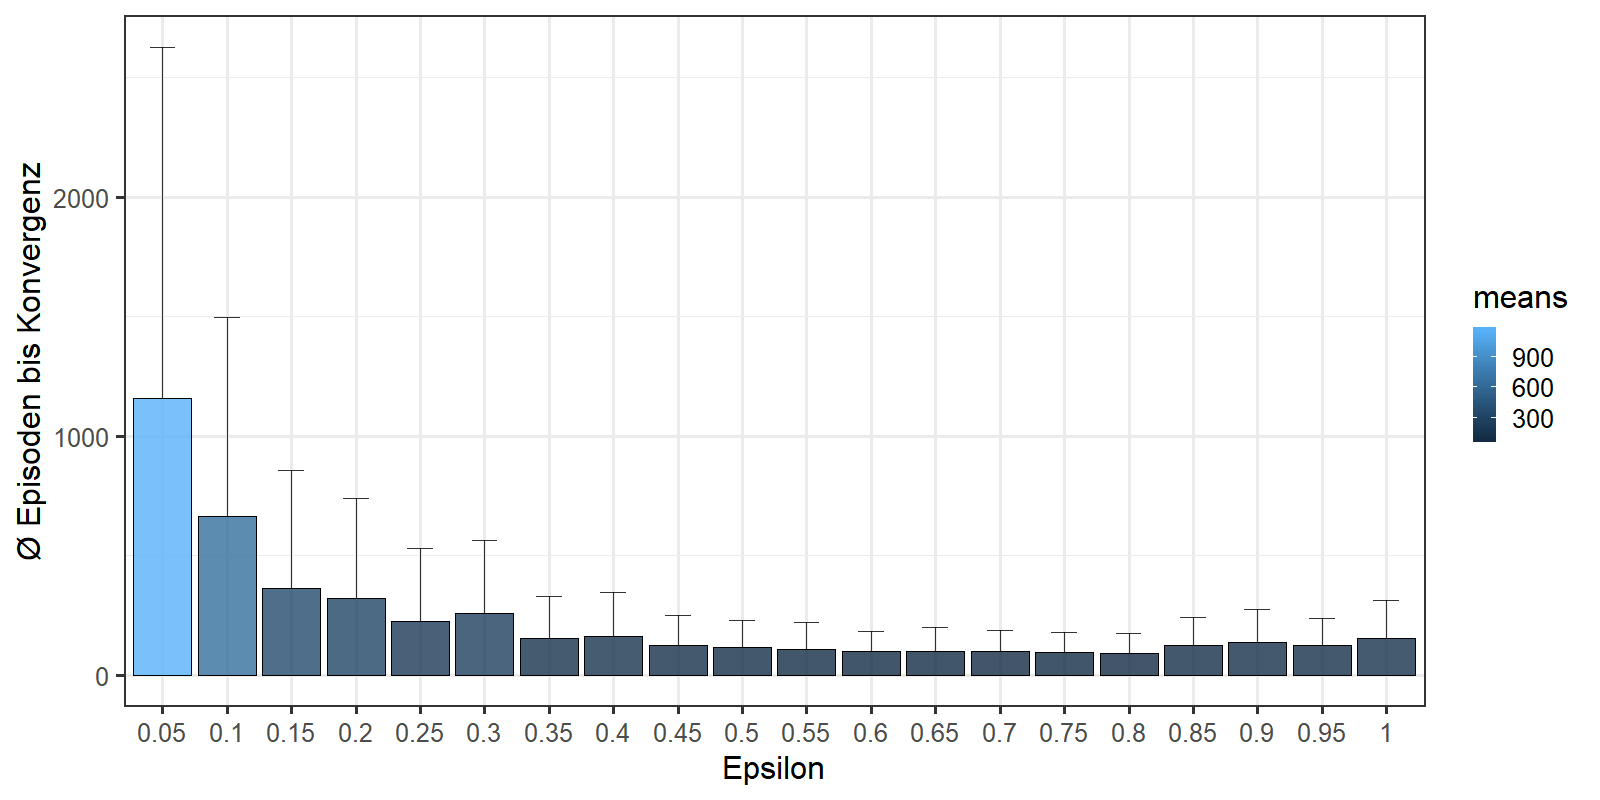
\includegraphics[width=\textwidth]{images/SimpleZ2B1MonteCarloA}
    \captionof{figure}{First-Visit Monte-Carlo, $Z_2, B_1$}
    \label{fig:test1}
\end{figure}

Deutlich zu erkennen ist, dass geringe Werte für $\epsilon$ einen negativen Effekt auf die benötigte Anzahl an Epsioden hat. Für $\epsilon = 0.05$ werden durschnittlich $1159$ Epsioden benötigt mit einer sehr hohen Standardabweichung von $1468$. Dies lässt sich vor allem damit erklären, dass die meisten Episoden damit enden, dass der Dino gegen das zweite Hindernis springt. Das liegt daran, dass die initalen Werte für jegliche Aktions-Nutzen 0 sind und mit Willkür zwischen ihnen gewählt wird, was dazu führt, dass der Dino immer wieder springt. Dieses Verhalten sorgt bei einer neuen Episode (zufällig) dafür, dass er das erste Hindernis überspringt, aber durch die Sprungabstände permanent mit dem zweiten Hindernis kollidiert. Für diesen Fall ergibt sich ein anhaltender Gewinn von $56$ (56 Zeitstempel bis zu der Kollision). Da die verwendete Belohnungsfunktion bewirkt, dass die Aktions-Nutzen einen positiven Wert annehmen, wenn sie in einer Episode ausgewählt werden, werden alternative Aktionen mit einer Wahrscheinlichkeit von $1-\epsilon$ nicht versucht. Je größer $\epsilon$, desto größer ist die Wahrscheinlichkeit, dass der Algorithmus aus seinem lokalen Maximum herausfindet und durch eine spezielle Aktionsreihenfolge lernt, das zweite Hindernis zu überspringen.
\par
Bemerkenswert ist, dass komplett zufälliges Handeln ($\epsilon = 1$) nur durschnittlich 155 Episoden benötigt, um zu konvergieren. Dies ist ein Hinweis darauf, dass das Problem in der Tat sehr simpel ist, weil der reine \textit{Brute-Force}-Ansatz nicht sonderlich schlechter abschneidet, als die besten Experimente ($0.5 <= \epsilon <= 0.8$ ) mit ungefähr 100 Episoden bis zu dem Erreichen der optimalen Strategie.

\par 
In Kapitel \ref{sec:JDbelohnungsfunktion} wurde erklärt, dass die Belohnungsfunktion für das TD-Learning anders modelliert werden sollte als für die MC-Methoden. Um herauszufinden, ob eine Konvergenz dennoch stattfinden kann, wurden die gleichen Bedingungen, also Zustandsmodellierung $Z_2$ und Belohnungsfunktion $B_1$, bei dem Q-Learning untersucht. Letztendlich ist der Unterschied zwischen der Belohnungsfunktion $B_1$ und der Belohnungsfunktion speziell für das TD-Learning $B_2$ lediglich eine Verschiebung um -1. Das Verhältnis zwischen der Belohnung für jeden Zeitstempel und der Belohnung bei der Kollision ist dasselbe.
\par 
Neben der Standardinitalisierung der Aktions-Nutzen auf den Wert 0, wird zudem untersucht, ob ein Standardwert von \textit{Integer.MAX\_VALUE} einen Unterschied verursacht.

\begin{figure}[H]
  \centering
  \begin{minipage}{.5\textwidth}
    \centering
    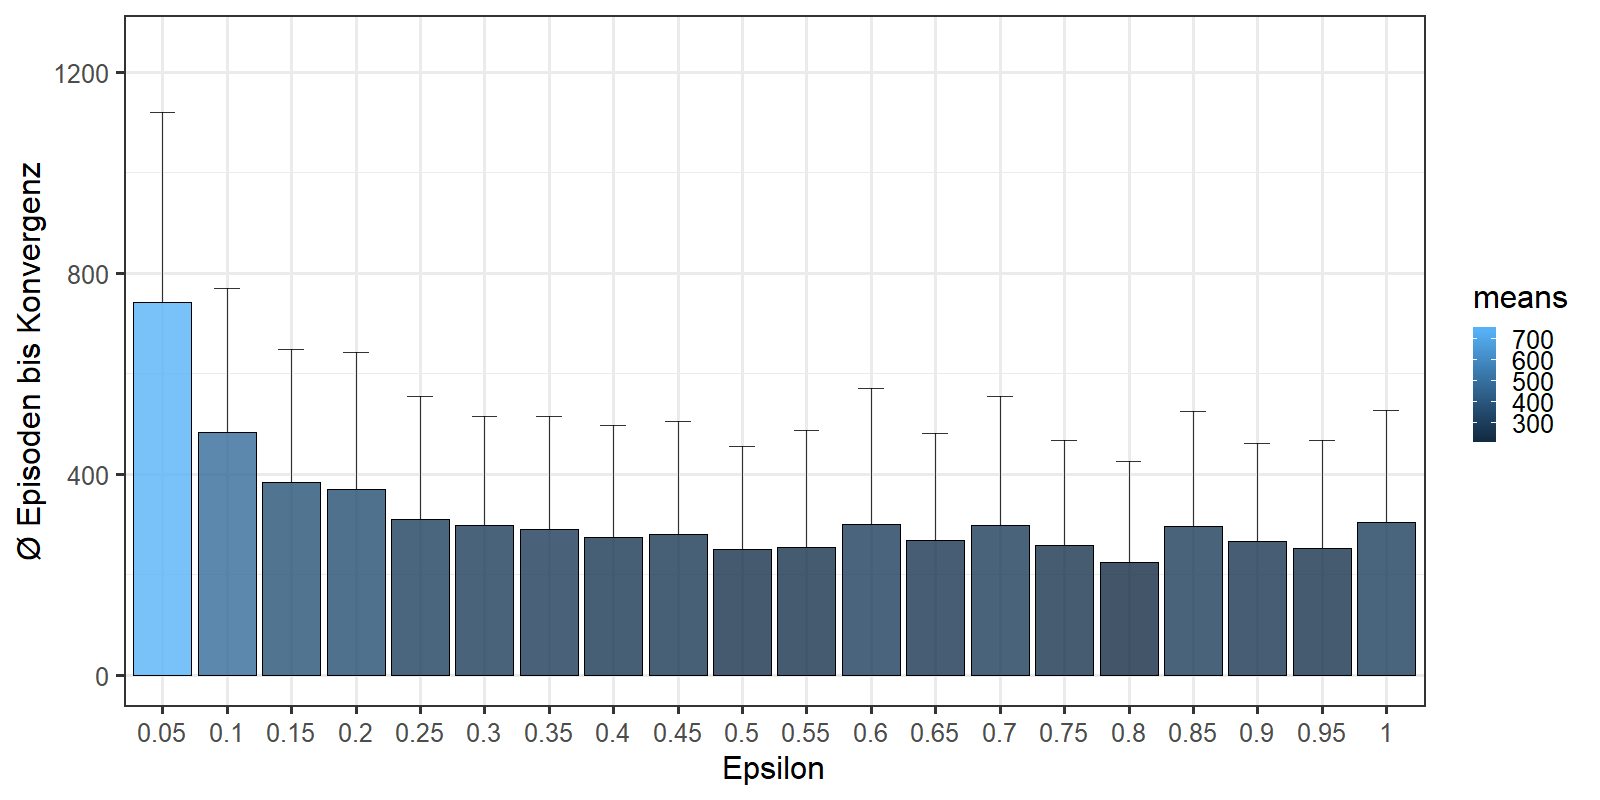
\includegraphics[width=\textwidth]{images/SimpleZ2B1QLearningA}
    \captionof{figure}{Q-Learning $Z_2, B_1$}
    \label{fig:test1}
  \end{minipage}%
  \begin{minipage}{.5\textwidth}
    \centering
    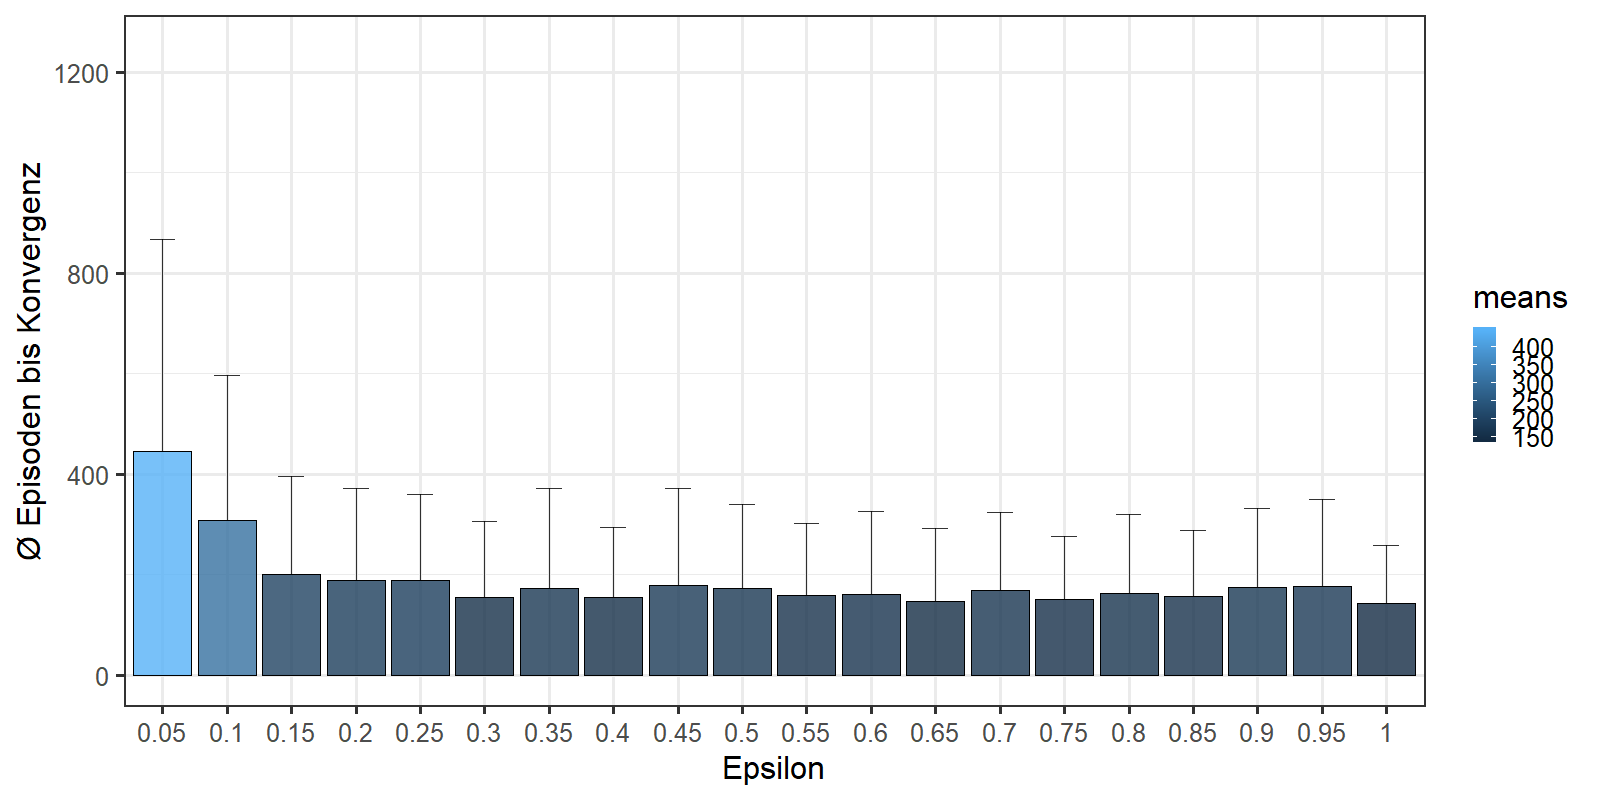
\includegraphics[width=\textwidth]{images/SimpleZ2B1QLearningMaxA}
    \captionof{figure}{Q-Learning, $Z_2, B_1$,maxQ}
    \label{fig:test2}
  \end{minipage}
\end{figure}
Die Ergebnisse zeigen, dass das Q-Learning in der Lage ist, mit der gleichen, für episodiale Lernmethoden zugeschnittene, Belohnungsfunktion zu konvergieren. Andersherum ist dies nicht möglich. Monte-Carlo Methoden unter Verwendung der Belohnungsfunktion $B_2$ können nicht konvergieren, da jegliche Aktions-Nutzen den Wert -1 annehmen.
\par 
Für den Initialwert 0 für neue Aktions-Nutzen konvergiert das Q-Learning im Vergleich zu der \textit{First-Visit} Monte-Carlo Methoden im Durschnitt langsamer. Der Durschnitt für die benötigten Episoden über alle Werte des Parameters $\epsilon$ für die MC-Methode beträgt 234, für das Q-Learning 320. Werden die Aktions-Nutzen allerdings mit dem \textit{Integer.MAX\_VALUE} initialisiert, dann ist das Q-Learning sogar performanter als die \textit{First-Visit} Variante der MC-Methoden, mit einem Durschnitt von 188 Episoden bis zu der Konvergenz. Die Initialisierung der Aktions-Nutzen mit sehr hohen Werten begünstig die Erkundung des Zustand- bzw. Aktionsraumes, da die realen Nutzen kleiner sind als die intialen Werte. Eine Aktualisierung bedeutet eine Verringerung der Aktions-Nutzen der ausgeführten Aktion, wodurch nicht ausgewählte Aktionen den größten Nutzen bei der nächsten Entscheidung beibehalten und mit einer Wahrscheinlichkeit von $1-\epsilon$ ausgewählt werden.
\par 

\subsubsection*{Angepasste Belohnungsfunktion für TD-Learning}
Wie wichtig es ist, die Belohnungsfunktion korrekt zu modellieren und das nicht nur im Bezug auf das eigentliche Problem, sondern auch auf den verwendeten Lernalgorithmus, zeigen die nachfolgenden Ergebnisse.
\par 
Anstatt positive Verhalten zu belohnen und für jeden Zeitstempel +1 zu vergeben wird bei der Belohnungsfunktion $B_2$ nur Fehlverhalten, die Kollision mit dem Hindernis, bestraft. Um die Summe der Belohnungen zu maximieren, wie es jeder RL-Algorithmus versucht, muss somit eine Kollision vermieden werden. Durch den Diskontierungsfaktor $\gamma = 0.99$ bekommt der Agent die \glqq Weitsicht\grqq{}, um Entscheidungssequenzen zu erlernen, die eine Kollision und damit den Erhalt einer negativen Belohnung verhindern. 
\par 
Die Anpassung der Belohnungsfunktion zeigt die Stärken der TD-Algorithmen \textit{Q-Learning} und \textit{SARSA}, die eine deutlich schnellere Konvergenz im Vergleich zu der \textit{First-Visit} MC-Methode bieten.

\begin{figure}[H]
    \centering
    \begin{minipage}{.5\textwidth}
      \centering
      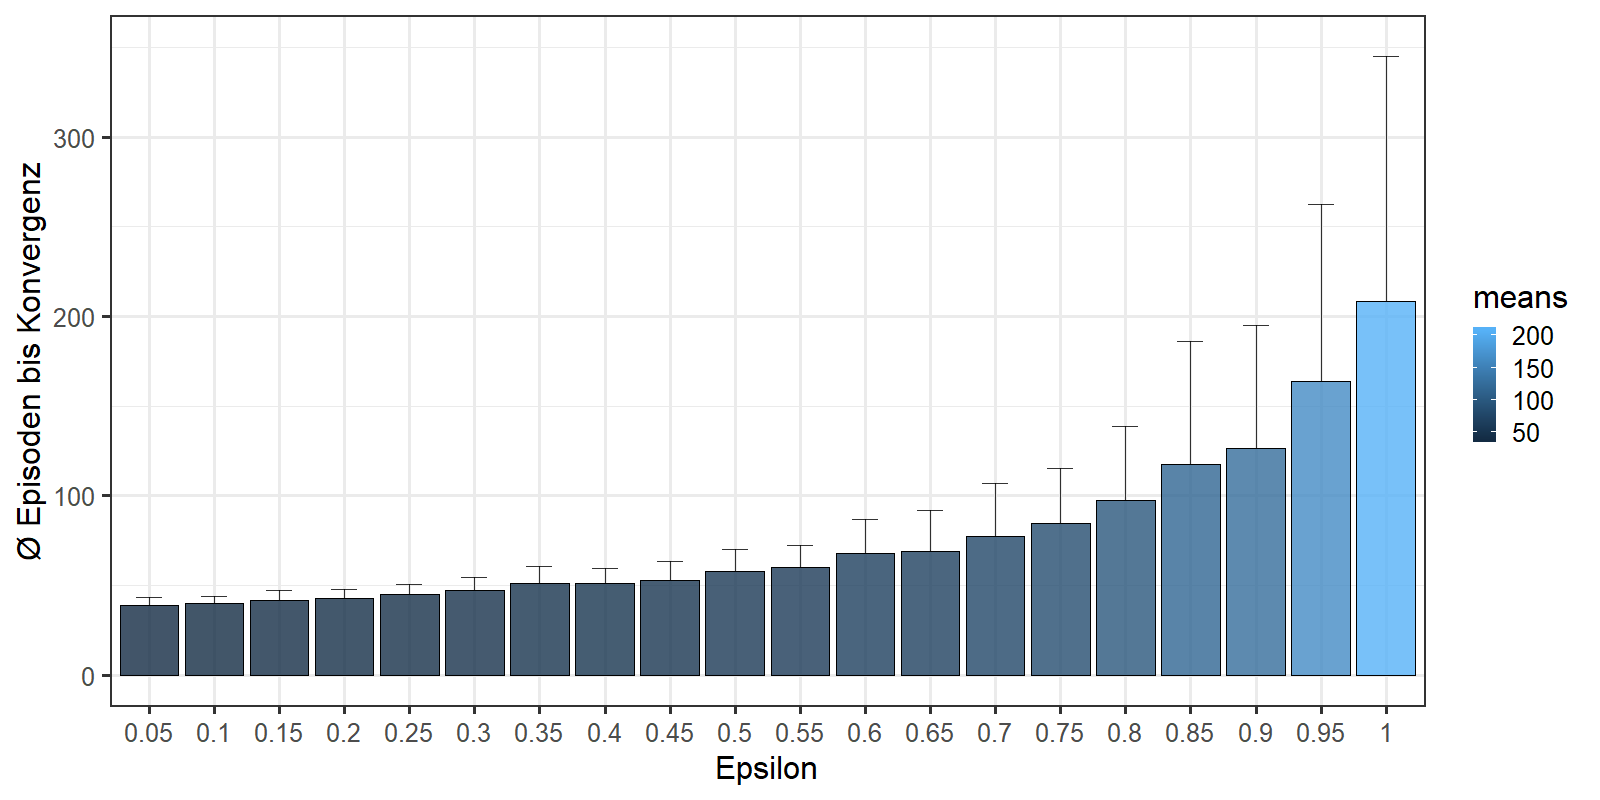
\includegraphics[width=\textwidth]{images/SimpleZ2B2QLearningA}
      \captionof{figure}{Q-Learning $Z_2, B_2$}
      \label{fig:test1}
    \end{minipage}%
    \begin{minipage}{.5\textwidth}
      \centering
      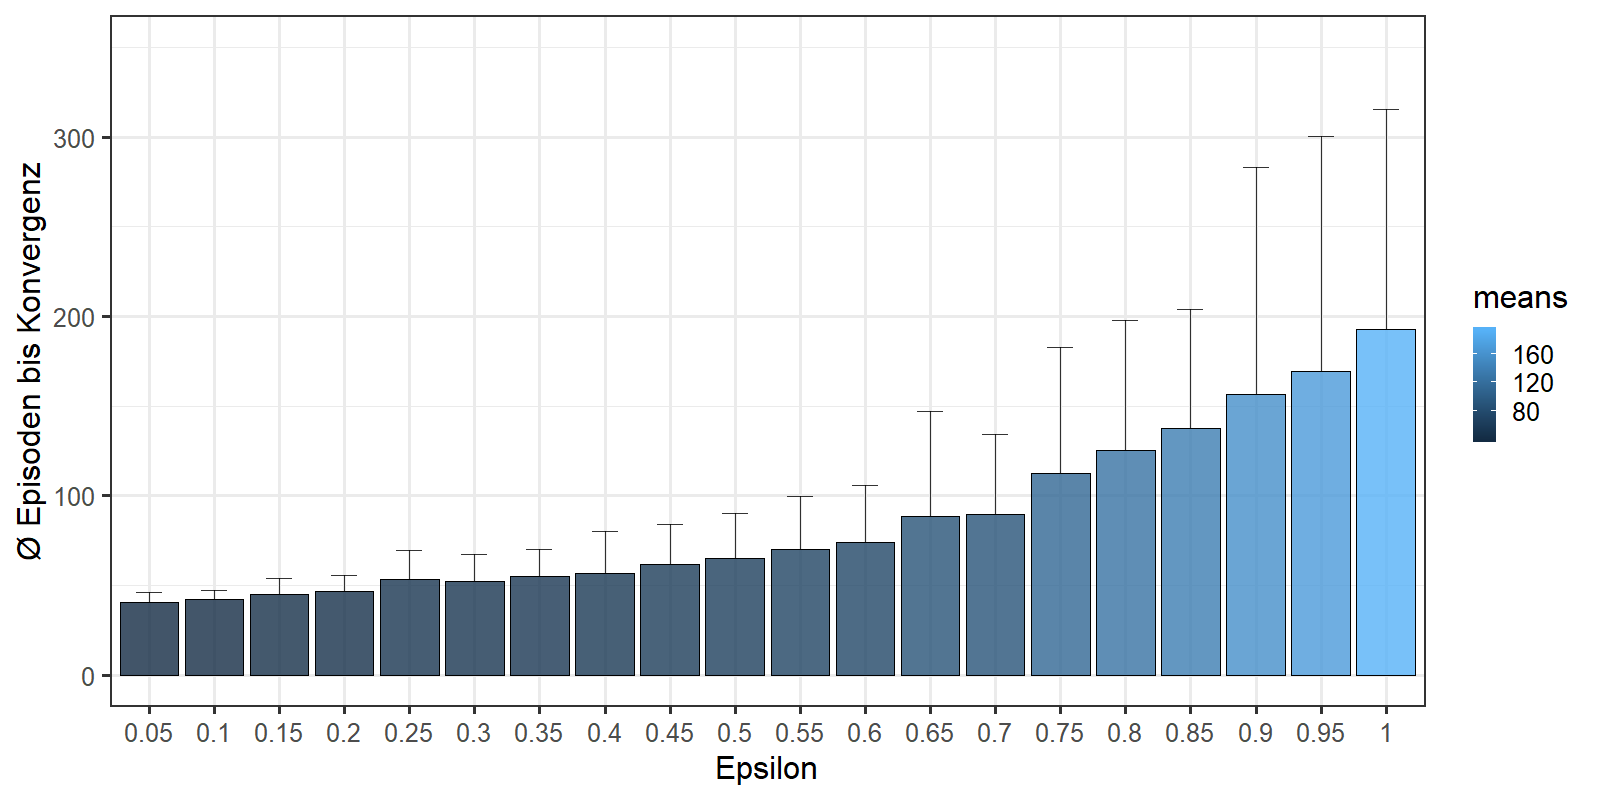
\includegraphics[width=\textwidth]{images/SimpleZ2B2SarsaA}
      \captionof{figure}{SARSA $Z_2, B_2$}
      \label{fig:test2}
    \end{minipage}
\end{figure}
Beide TD-Algorithmen konvergieren unter Verwendung von $B_2$ deutlich schneller als die MC-Methode, wobei \textit{Q-Learning} mit 77 durschnittlichen Episoden marginal bessser abschneidet als \textit{SARSA} mit 86 Episoden. Der deutliche Unterschied liegt im umgekehrten Trend, der durch den Paramter $\epsilon$ gegeben ist. Hierbei steigt der Aufwand bis zu Findung der optimalen Strategie mit größer werdenden $\epsilon$. Beide Algorithmen erreichen bei $\epsilon = 0.05$ die schnellste Konvergenz (39 respektive 40 benötigte Episoden). Grund hierfür ist die Modellierung der Belohungsvergabe und den daraus resultierenden Aktions-Nutzen. Je geringer $\epsilon$, desto konsistenter wird die Aktion mit dem aktuell höhsten Nutzen ausgewählt. Aktionen die bereits  ausgeführt worden sind und letztendlich zu einer Kollision geführt haben, nehmen einen negativen Wert an, wodurch alternative Aktionen passiv zu der vermeintlich besten Aktion werden. 
\par 

\subsubsection*{Fehlen der \glqq inJump\grqq{} Information}
Der naive Erstansatz des Autors für die Zustandsmodellierung des Jumping Dino \textit{Simple} Lernszenarios bestand aus der Annahme, dass der Abstand zwischen Dino und Hindernis ausreichend sei, um das Problem lösen zu können. In diesem Unterabschnitt wird diskutiert, ob diese Information wirklich gegeben sein muss, bzw. warum es ohne sie nicht zu einer optimalen Entscheidungsfindung kommen kann.
\par 
Zu Beginn wurde angenommen, dass das Jumping Dino \textit{Simple} Problem eine einfache Schwellwertsuche sei. Der Dino muss dabei nur den korrekten Abstand zu dem Hindernis finden, bei dem er die Aktion \textit{JUMP} ausführen muss, bei allen anderen Abständen genügt die Aktion \textit{NOTHING}. In der Theorie ist das auch der Fall, deswegen warf sich das Rätsel auf, warum die \textit{First-Visit} Monte-Carlo Methode unter dieser Zustandsmodellierung nicht zu einer optimalen Strategie konvergieren konnte. In nur durschnittlich 7 von 100 Experimenten pro Paramterwert $\epsilon$ findet die \textit{First-Visit} Variante das optimale Verhalten.
\par 
Bei genauerer Betrachtung lässt sich jedoch der Grund für hierfür finden. Der Dino schafft es beständig über das erste Hindernis zu springen. Dabei erfährt er bereits alle 31 möglichen Zustände. Kommt das zweite Hindernis auf ihn zu, so erlebt er erneut sämtliche Zustände. Entscheidend ist, dass die \textit{First-Visit} Variante nur für den ersten Besuch eines Zustands-Aktions-Paares die Aktions-Nutzen anpasst, also für alle Paare für die Begegnung mit dem ersten Hindernis. Durch den Sprung über das erste Hindernis verschieben sich jedoch die Zeiträume, in dem der Dino sich im Sprung befindet und weil er durch die fehlende Information \glqq inJump\grqq{} keine Möglichkeit hat zu wissen, ob die Aktion \textit{JUMP} tatsächlich einen Sprung auslösen kann oder er sich z.B. gerade im Fall befindet, scheitert er unaufhörlich an dem zweiten Hindernis.
\par 
Die \textit{First-Visit} Variante ist somit nicht auf diese konkrete Aufgabenstellung anwendbar. Doch schafft es die abgewandelte \textit{Every-Visit} Variante, bei der alle Zustands-Aktions-Paare einer gesammelten Episode aktualisiert werden? \par 
Die Antwort lautet \textit{ja}, jedoch mit einer sehr hohen Varianz bzw. Standardabweichung zwischen den einzelnen Durchläufen bei gleichem $\epsilon$. Beispielsweise gibt es in der Testgruppe $\epsilon = 0.3$ Durchläufe, die bereits nach nur 7 Episoden konvergiert sind und solche, die bei einem anderen \textit{Random Seed} jedoch über 65000 Episoden benötigen.

\begin{figure}[H]
  \centering
  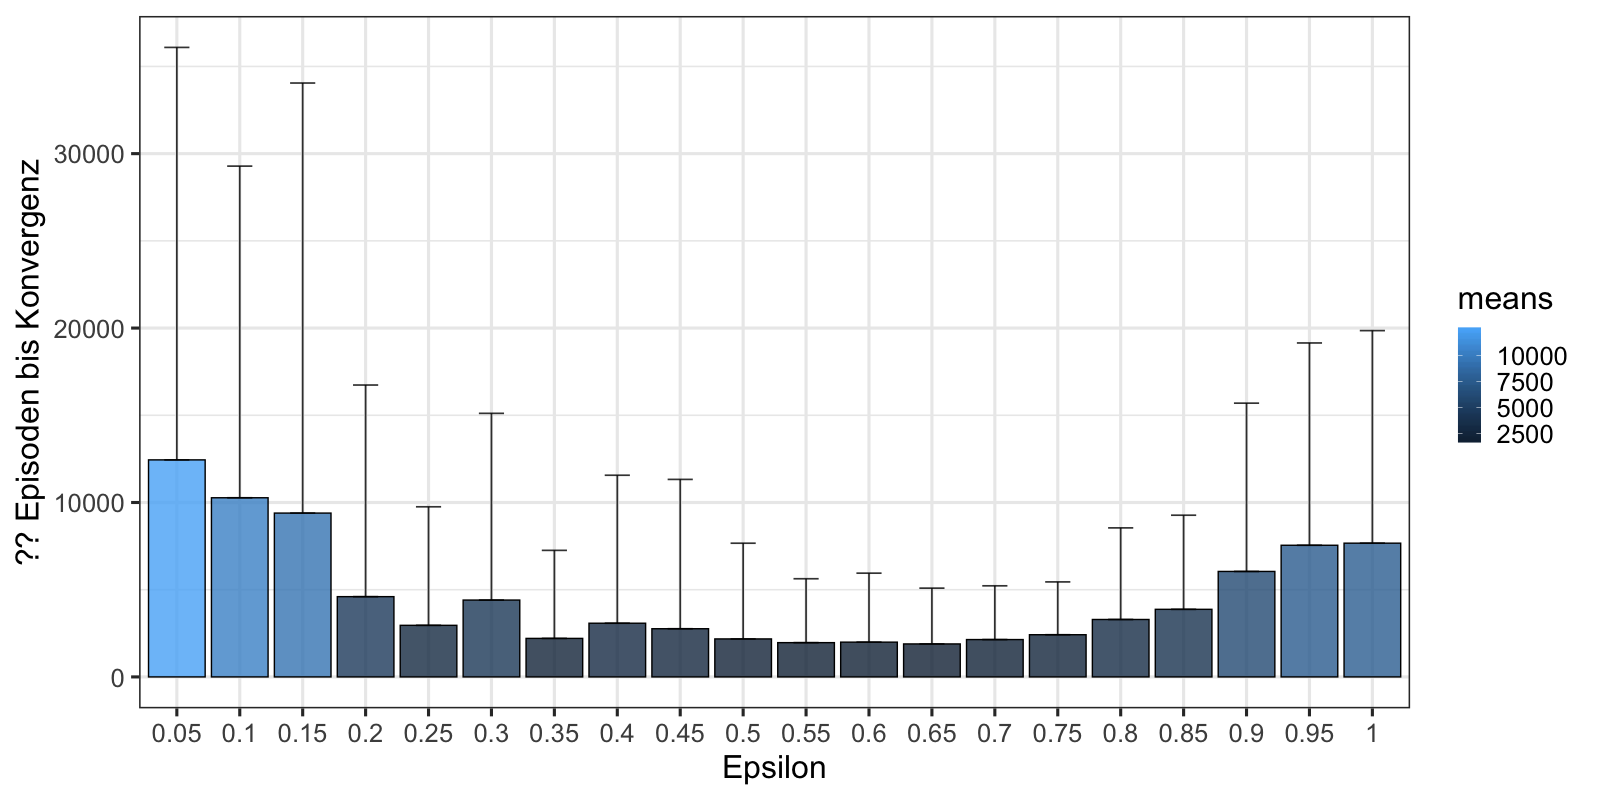
\includegraphics[width=\textwidth]{images/SimpleNoJumpEveryVisitMCA}
  \captionof{figure}{Every-Visit Monte-Carlo, $Z_1, B_1$}
  \label{fig:test1}
\end{figure}
 
\textit{Q-Learning} und \textit{SARSA} sind ebenfalls in der Lage, ohne die Information, ob sich der Agent im Sprung befindet oder nicht, zu optimalen Verhalten zu konvergieren. Im Gegensatz zu dem \textit{Every-Visit} Algorithmus konvergieren diese beiden TD-Algorithmen allerdings deutlich schneller.\textit{Every-Visit} benötigt durschnittlich 4656 Episode im Vergleich zu dem {Q-Learning}, welches nur durschnittlich 210 Epsioden benötigt. Des Weiteren ist dieses konkrete Szenario das einizige, bei dem \textit{SARSA}, mit durschnittliche 184 Episoden, besser abschneidet als das \textit{Q-Learning}. In allen anderen Versuchen zeigte das \textit{off-policy} Lernen ein schnelleres Konvergenzverhalten.
\par 
Auffällig ist, dass $\epsilon$ nur einen sehr geringen Einfluss auf das Konverhalten beider Algorithmen hat. 

\begin{figure}[H]
    \centering
    \begin{minipage}{.5\textwidth}
      \centering
      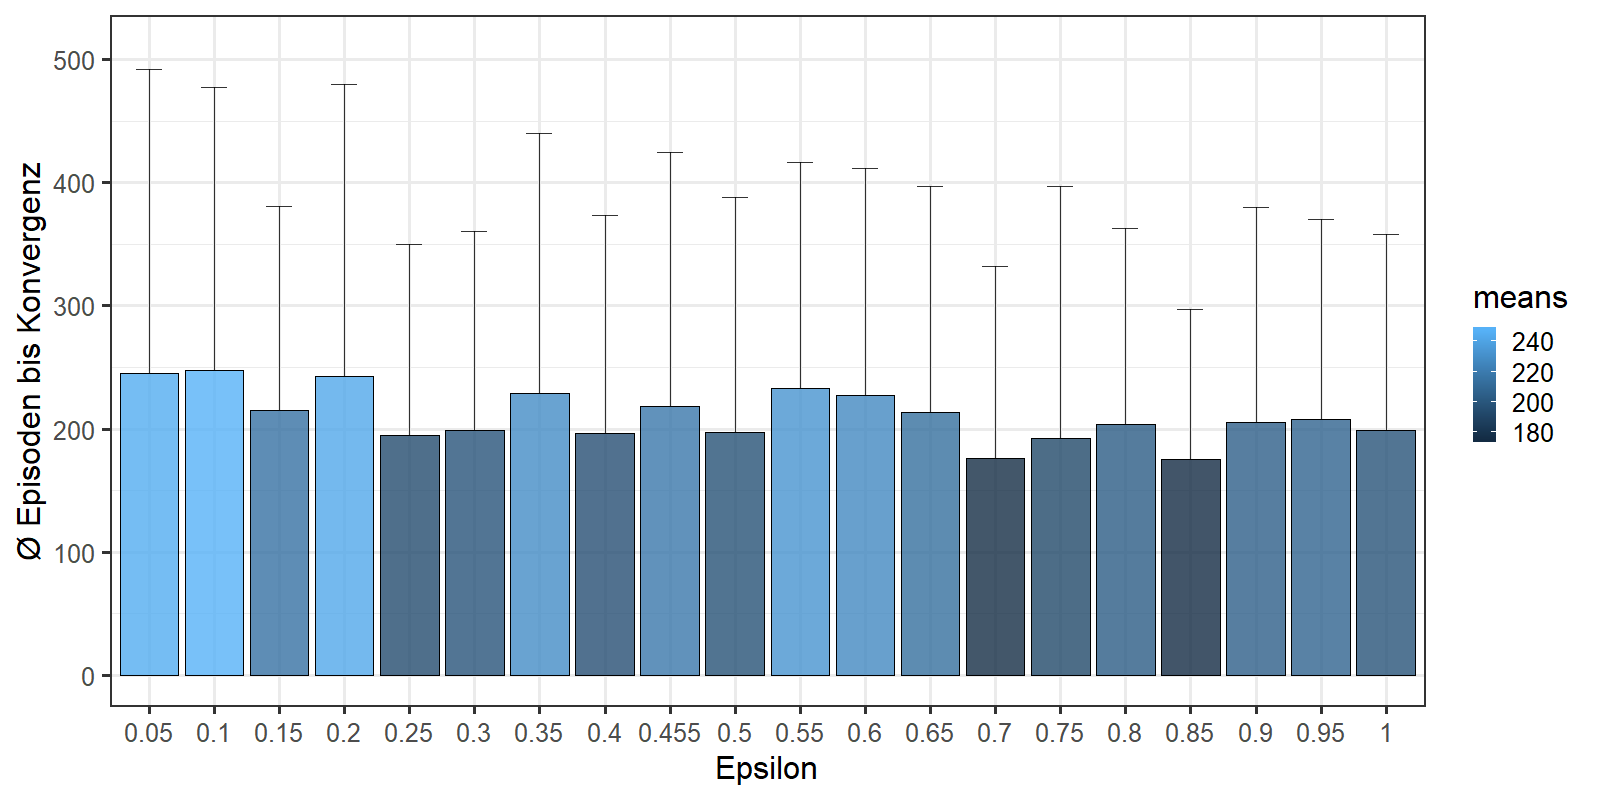
\includegraphics[width=\textwidth]{images/SimpleZ1B2QLearningA}
      \captionof{figure}{Q-Learning $Z_1, B_2$}
      \label{fig:test1}
    \end{minipage}%
    \begin{minipage}{.5\textwidth}
      \centering
      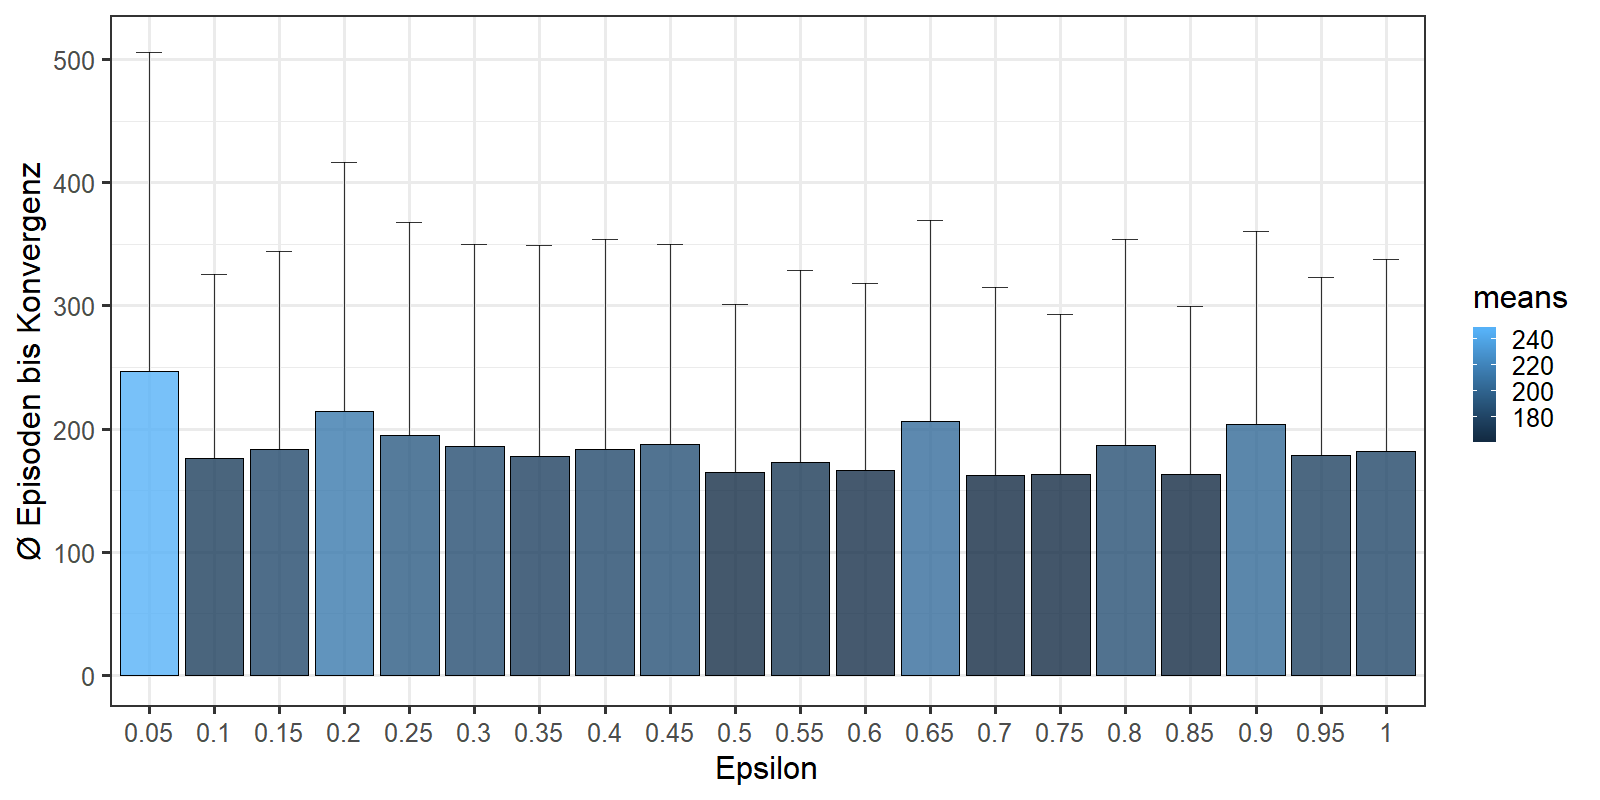
\includegraphics[width=\textwidth]{images/SimpleZ1B2SarsaA}
      \captionof{figure}{SARSA $Z_1, B_2$}
      \label{fig:test2}
    \end{minipage}
\end{figure}

\subsubsection*{Einfluss einer detaillierteren Belohnungsfunktion}
Als Letztes wurde getestet, ob eine detaillierte Belohnungsfunktion die Konvergenzgeschwigkeit erhöhen. Hierzu wurde ebenfalls eine Belohnung von -1 an den Agenten verteilt, wenn dieser versucht im Sprung die Aktion \textit{JUMP} auszuführen, da diese keinen Effekt hat. Die Annahme ist, dass das \textit{Q-Learning} dadurch einen deutlich geringen Zustands- und Aktionsraum für die Auswahl der optimalen Entscheidungssequenz zur Verfügung hat, da es direkt  die Aktion \textit{JUMP} als suboptimal verwirft, sobald einmal die Aktion \textit{JUMP} in einem Zustand mit \glqq inJump\grqq{} ausgeführt wird. 
\begin{figure}[H]
    \centering
    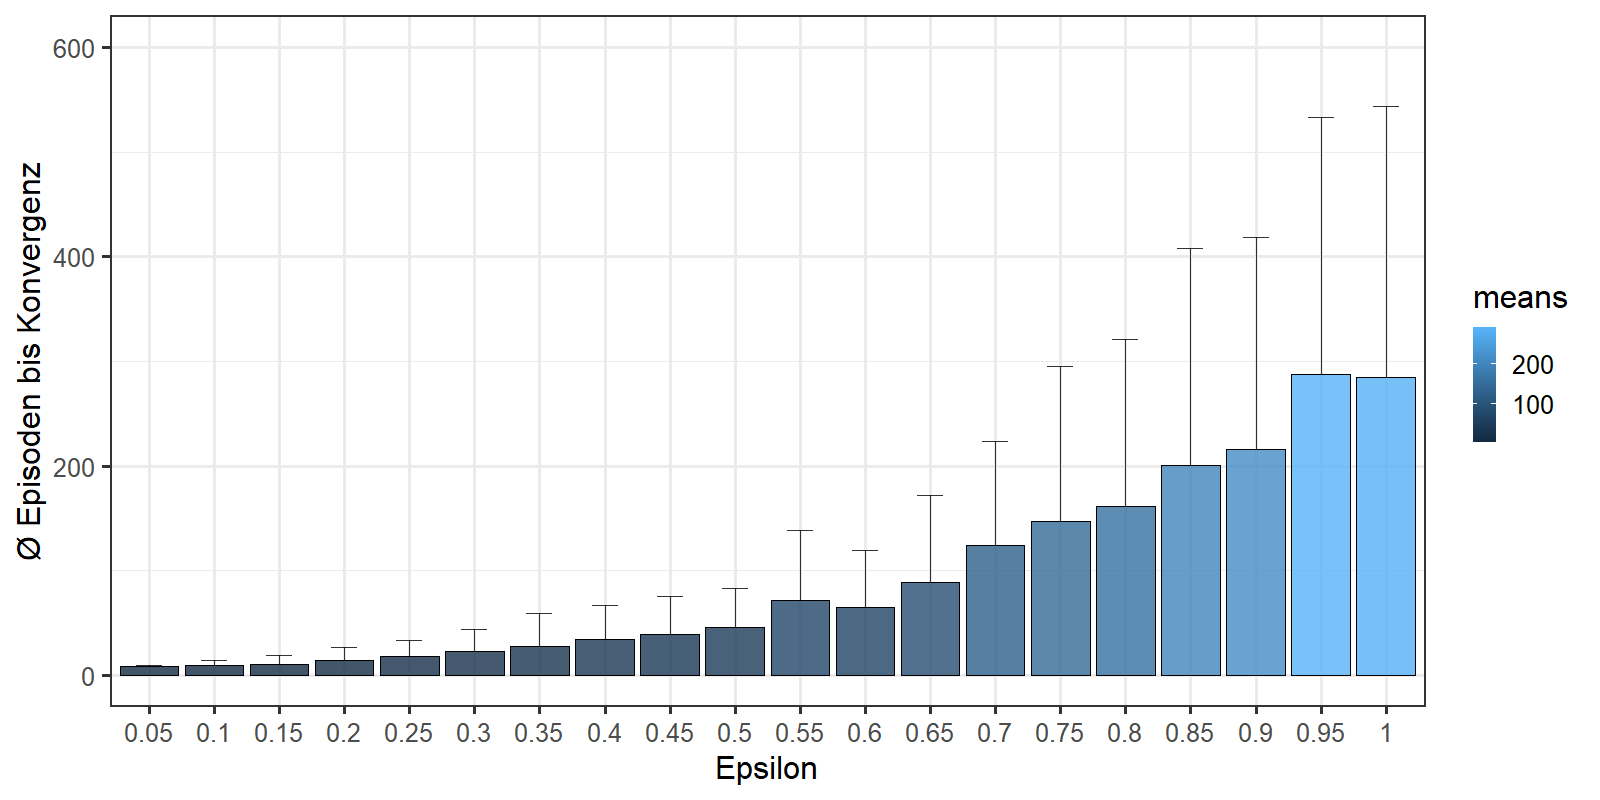
\includegraphics[width=\textwidth]{images/SimpleZ2B4QLearningA}
    \captionof{figure}{Q-Learning $Z_2, B_4$}
    \label{fig:test1}
\end{figure}
Mit nur 8 durschnittlichen Episoden bis zu dem Erreichen des optimalen Verhaltens bei einer Standardabweichung von $1.6$ ist diese Kombination von Lernalgorithmus, Zustands- und Belohnungsfunktionmodellierung mit Abstand die effizienteste.

\subsubsection{Konvergenzverhalten \textit{Advanced} Variante}
Um den Aufwand zur Lösung des Jumping Dino Spiels zu vergrößern, wurde eine \textit{Advanced} Variante in Kapitel 4.2.1 vorgestellt. In dieser Version bewegen sich die Hindernisse zufällig mit vier unterschiedlichen Geschwindigkeiten und erscheinen  mit vier unterschiedlichen Abständen. Statt 116 Zustands-Aktions-Paaren, müssen nun 4146 Paare gespeichert und bewertet werden.
\par 
Betrachtet wird zunächst die \textit{First-Visit} Variante der Monte-Carlo Methoden, die ausschließlich auf Basis von vollständig gesammelten Episoden lernen kann.
\begin{figure}[H]
    \centering
    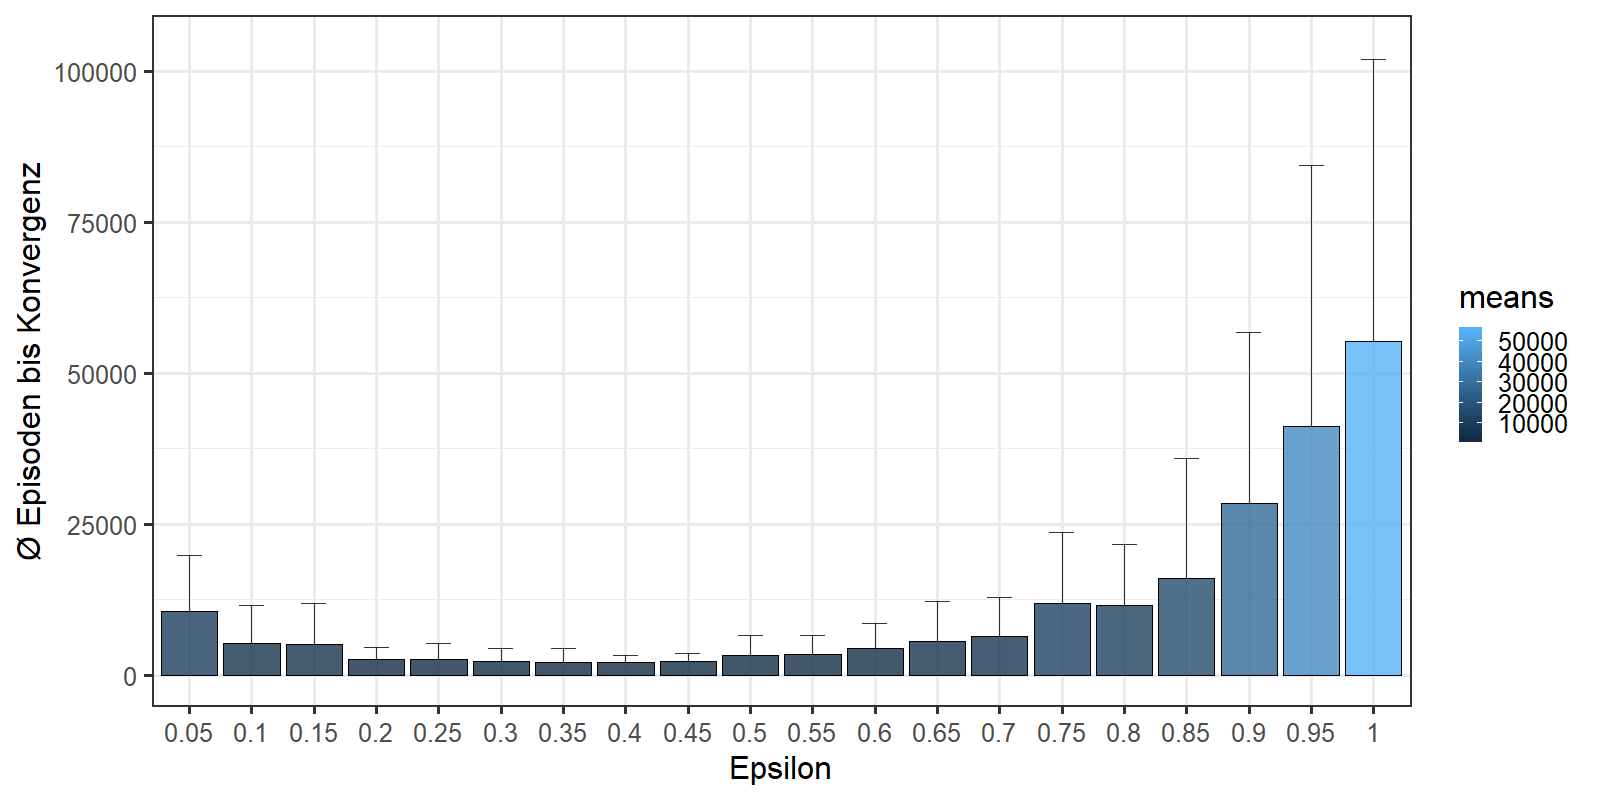
\includegraphics[width=\textwidth]{images/AdvancedZ3B1MonteCarloA}
    \captionof{figure}{First-Visit Monte-Carlo $Z_3, B_1$}
    \label{fig:test1}
\end{figure}
Im Vergleich zu der \textit{Simple} Variante, bei der niedrige Werte für $\epsilon$ am langsamsten konvergierten, ähnelt die Verteilung der, der TD-Algorithmen, die mit höherer Zufallswahrscheinlichkeit $\epsilon$ deutlich mehr Episoden benötigten, um zu optimalen Verhalten zu gelangen. Durschnittlich benötigte der \textit{First-Visit} Algorithmus 11155 Episoden und lieferte bei $\epsilon = 0.4$ das beste Ergebnis mit 2079 Episoden bei einer Standardabweichung von 1190. 
\par 
Das \textit{Advanced} Problemszenario ist in sofern komplexer, da deutlich längere Entscheidungssequenzen bewertet und optimiert werden müssen. Lange Sequenzen wie in diesem Beispiel verdeutlichen die threoretischen Annahmen für Werte von $\epsilon$. Ist $\epsilon$ zu niedrig gewählt, dann sinkt die Effizienz. In diesem konkreten Experiment äußern sich Werte kleiner gleich $0.15$ negativ auf das Konvergenzverhalten. Niedrige Werte für $\epsilon$ bewirken, dass aktuell optimal erscheinende Entscheidungssequenzen nur langsam angepasst werden, um letztendlich verbesserte Sequenzen zu erzeugen. Andersherum sorgen hohe Werte für $\epsilon$ dafür, dass bisher optimale Entscheidungsketten frühzeitig durch eine suboptimal, zufällig gewählte Aktion unterbrochen werden und kein zusätzliches Lernen durch die aktuelle Episode erreicht werden kann. Dabei ist $\epsilon = 1$ ist der Extremfall, bei dem jegliche Kombinationen von Aktionsreihenfolgen zufällig erzeugt werden und lediglich die Bewertung dieser zu optimalen Verhalten führt. Für diesen Fall wird also nur das Vorhersageproblem gelöst und das Konzept der \textit{Generalized Policy Iteration (GPI)} verworfen, weil keine Strategieverbesserung stattfinden kann, da sich die Strategie nicht an den Aktions-Nutzen orientiert, sondern ausschließlich willkürlich agiert.
\subsubsection*{Anwendung der TD-Algorithmen}
Die Ergebnisse zu dem Konvergenzverhalten bei der \textit{Simple} Variante des Jumping Dino Spiels haben gezeigt, dass die TD-Algorithmen \textit{Q-Learning} und \textit{SARSA} deutlich effizienter lernen als die MC-Methoden. Daher ist anzunehmen, dass sie auch in der \textit{Advanced} Variante eine bessere Performance zeigen.
\par 
In der praktischen Anwendung der beiden TD-Algorithmen stellte sich jedoch heraus, dass beide nicht in der Lage sind, zu optimalen Verhalten zu konvergieren. Dabei ist es unerheblich, welche Variante der Belohungsmodellierung gewählt wird. Auf eine aufwendige  Untersuchung, welche konkreten Ursachen für dieses Versagen verantwortlich sind, wurde aus zeitlichen Gründen verzichtet. Neben den unterschiedlichen Belohnungsfunktionen wurden auch zahlreiche Kombinationen von Diskontierungsfaktor $\gamma$ und Lernrate $\alpha$ getestet, ohne Erfolg.
\par 

\subsubsection{Zusammenfassung}
In diesem Kapitel wurden viele unterschiedliche Problemszenarien unter Verwendung verschiedener RL-Algorithmen untersucht. In der \textit{Simple} Variante des Jumping Dino Spiels zeigten die \textit{Temporal-Difference Learning} Algorithmen ein deutlich schnelleres Konvergenzverhalten. Vor allem bei der angepassten Belohnungsfunktion $B_4$, die wirkungslose Aktionen direkt bestraft, zeigte das \textit{Q-Learning} seine Stärken.
\par 
Interessante Erkenntnisse konnten über die unterschiedliche Vorgehensweise zwischen den beiden MC-Methoden \textit{First-Visit} und \textit{Every-Visit} gesammelt werden. Nur die \textit{Every-Visit} war in der Lage zu optimalen Verhalten zu konvergieren, ohne die Information zu erhalten, ob der Dino sich derzeit im Sprung befindet oder nicht.
\par 
Dass theoretisches Grundlagenwissen über die Arbeitsweise der beiden Algorithmengruppen Monte-Carlo und \textit{Temporal-Difference} essentiell für eine Bewertung ist, welche Algorithmen für eine bestimmte Aufgabenstellung anwendbar sind, offenbart die Anwendung dieser auf die \textit{Advanced} Variante. Bei klar definierten Episoden kann die Anwendung der MC-Methoden präferiert werden, da die Vorgehensweise bzw. die Berechnung der Aktions-Nutzen leichter zu durchdringen ist als bei dem TD-Learning, die das Konzept eines Terminalzustands nicht benutzen. Zudem sind die MC-Methoden in der Lage bei der \textit{Advanced} Variante zu optimalen Verhalten zu konvergieren, die TD-Algorithmen jedoch nicht. 